% Subsection 4.3: MOPS

\subsection{Moving Object Prediction System (MOPS)}
\label{sApps-mops}

DC2 integrated the night-time functionality of MOPS (``NightMOPS''),
which consists of predicting locations of known objects expected to
appear in images.  This is done concurrently with image processing,
with the intent of concurrently reporting both detected objects and
predicted objects to the Association Pipeline on a per-image basis.
This process is distributed trivially by distributing responsibility
for subsets of the set of known objects between multiple slices in the
NightMOPS Pipeline.

\subsubsection{MOPS Preparations for DC2}
In full LSST, the day-time functionality of MOPS (DayMOPS) involves
processing large sets of detections into a catalogue of orbits.
Additionally, each day DayMOPS will be responsible for making two or
more ephemeris predictions for all known orbits for the coming night.
To prepare a catalogue and collection of ephemerides which was similar
to that expected in full-scale LSST, we fed the Minor Planets Center
catalogue of detections into DayMOPS.  The DayMOPS software generated
a catalogue of 159357 orbits based on 29779380 detections.  Prior to
DC2, three ephemeris points were predicted per orbit, per night for
which we had image data, a total of 87008922 ephemerides.  The
ephemeris points were predicted at midnight, 4 PM before that midnight
and 8 AM after that midnight, and stored in the central LSST database.

\subsubsection{NightMOPS Within DC2}

\paragraph{}
NightMOPS was implemented as an Application Pipeline, implemented
entirely in \code{Python}.  The workload was distributed between
Pipeline Slices, each of which were responsible for subsets of the
total objects.

NightMOPS received its input from the DC2 Harness via the Events
system, which would announce a field of view and time as image
processing for those images began.  On receiving this Event, each
NightMOPS Slice would concurrently query the ephemeris collection
generated by DayMOPS for ephemeris points (and their associated error
ellipses) corresponding to the evening of the image and the Slice's
assigned object IDs.  Slices would then prune objects which would not
pass nearby the field of view at that time and ignored them.  The
positions of the remaining objects were quadratically interpolated
from their three associated ephemerides.  These positions and their
associated object IDs were then passed on to the Association Pipeline
via the persistence framework and the database, with an Event passed
to the Association Pipeline informing it of the availability and
location of the data.


\subsubsection{Results}
NightMOPS predicted 25 objects which were detected in images during
the DC2 runs.  This small number of matches seems to be a result of
the limited number of objects detected in the MPC database and the
areas of sky in the images we chose for DC2.  All of our interpolated
ephemeris locations  were very close to the actual observed
detections, an average of 5.8 arcsec in error.  The maximum
distance between predicted location and observed location was
10 arcsec; the minimum was 1 arcsec.   An example detection of a MOPS
predicted object position is shown in \Fig{MOPSPredImage}.

\begin{figure}[htb]
\begin{center}
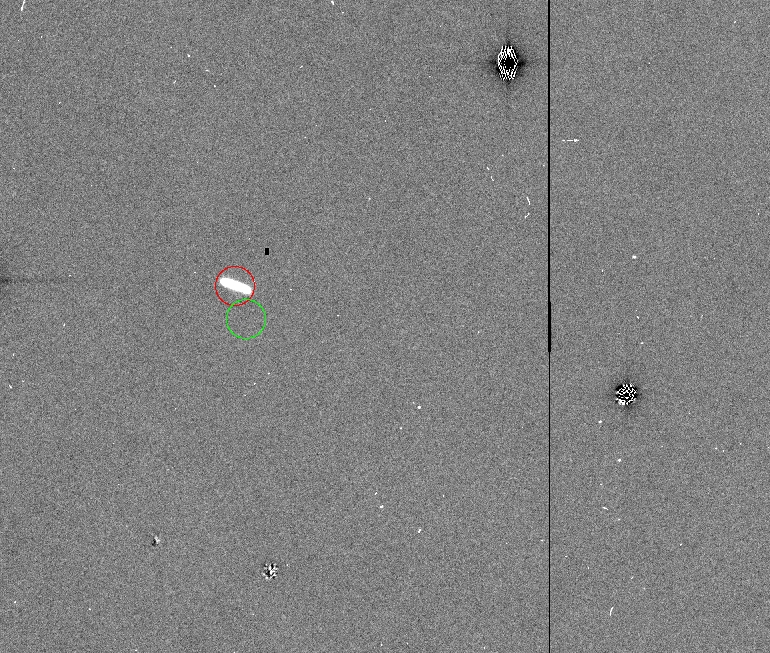
\includegraphics[height=60mm] {figures/MopsPred_rlp0130_705197}
\caption{Detection of a MOPS predicted solar system object in DC2.
The object has orbit\_id=41904, and was detected in Visit 705197.  The
green circle is centered on the predicted position, while the red
circle is centered on the detected position, which is about 6 arcsec away.}
\label{MOPSPredImage}
\end{center}
\end{figure}


%\subsubsection{Performance}
%NUMBERS and some OLD BENCHMARKS
%The majority of this time was dominated by database query and transfer.  This time was relatively small %compared to the time taken by image processing; NightMOPS was far from a bottleneck in DC2.

\subsubsection{Issues and lessons learned}

MOPS proved itself capable of night-time operation which met or
exceeded our performance demands.  Further, the DC2 preparation
demonstrated the functionality of the DayMOPS system for identifying
objects from sets of detections.  Though our number of matches between
ephemeris predictions and observed objects was somewhat small, this
was limited by factors outside of our control, including the currently
limited set of known asteroids.

The most significant problem within NightMOPS was that the predicted
error ellipses for objects were very large (average semi-minor axis:
1806.64 arcsec, average semi-major axis: 2947.12), especially when
contrasted with the average distance from detected object to predicted
ephemeris location (6 arcsec).  We see several possible causes for
this problem, particularly the ephemeris prediction libraries we used
to generate the orbital covariance matrices, which were provided to us
by the NASA Jet Propulsion Laboratory, or our own libraries which
convert from covariance matrices to error ellipses.  We are continuing
to investigate this problem and plan to address it in DC3.


It is also of note that database access time during NightMOPS
operation will likely decrease in the future: in LSST, we will only
need to query a table containing ephemeris for the current night, not
for a large set of nights as in DC2.  Further, small preliminary
experiments have found that changing our SQL query syntax can result
in as much as a fifty-fold increase for NightMOPS database queries.
As database query was the major factor in DC2 performance of
NightMOPS, we can expect NightMOPS to perform far better in DC3 and
full-scale LSST than we observed in DC2.

\subsubsection{Conclusions}
Though the small number of NightMOPS predictions to detected object
matches in DC2 was a small disappointment, DC2 proved a convincing
test of the NightMOPS subsystem, demonstrating both correctness and
high performance.  Further, we can realistically expect massive
improvements in performance, making a strong argument that even as
other Pipelines improve in performance, NightMOPS will not become a
bottleneck.

A further issue related to the JPL code is that it is only licensed
for use within the U.S.~and within the LSST consortium. We are 
exploring options for relaxing these restrictions or replacing
the JPL code with equivalent code (Milani or Tricarico).
